%-----------------------------------------------------------------
%	FORMULARI
%	!TEX root = ./main.tex
%-----------------------------------------------------------------
\section{\mytitle}
% TODO: other useful constants
%-----------------------------------------------------------------
\subsection{Transformada de Fourier}
\begin{align*}
	F(u,v) = \TF{f(x,y)} = \int f(x,y) e^{-i 2\pi (xu+yv)} \dd{x} \dd{y} \\
	f(x,y) = \TFI{F(u,v)} =\int F(u,v) e^{i 2\pi (xu+yv)} \dd{u} \dd{v}
\end{align*}
%
% \subsubsection*{Propietats}
\begin{align*}
\begin{gathered}
	\TF{f(x-x_{0},y-y_{0})} = F(u,v) e^{-i 2\pi (x_{0}u+y_{0}v)} \\
	\mc{F}^{0} = \bbid \qc \mc{F}^{1} = \mc{F} \qc \mc{F}^{2} = \mc{P} \qc \mc{F}^{3} = \mc{F}^{-1} \qc \mc{F}^{4} = \bbid \\
	f(ax, by) \mapsto \frac{1}{\abs{a}\abs{b}} F\qty(\frac{u}{a},\frac{v}{b}) \\
	\TF{f\sast(x,y)} = F\sast(-u,-v) \\
	\text{conv}: g(x) = f(x) \otimes h(x) = \int f(\alpha) \vdot h(x- \alpha) \dd{\alpha} \\
	\TF{f \otimes h} = F \vdot H \qc \TF{f \vdot h} = F \otimes H \\
	\text{corr}: g(x) = f(x) \ast h(x) = \int f(\alpha) \vdot h\sast(\alpha - x) \dd{\alpha} \\
	\TF{f \ast h} = F \vdot H\sast \qc \TF{f \vdot h\sast} = F \ast H \\
	% \pdv[k]{f(x)}{x} = \int(i 2\pi u)^{k} F(u) e^{i2\pi ux} \dd{u} \quad \Rightarrow \text{res. freq.} \\
	\TF{\pdv[k]{f(x)}{x}} = (i 2\pi u)^{k} F(u) \quad \Rightarrow \text{ressaltat freq.}
\end{gathered}
\end{align*}

% \subsubsection*{Llista de transformades}
\begin{align*}
	\delta &\leftrightarrow 1 \\
	\delta(x-a) + \delta(x+a) &\leftrightarrow \cos \,(\text{o } \sin) \\
	\uparrow \_ \uparrow \_ \uparrow &\mapsto \uparrow \_\_ \uparrow \_\_ \uparrow \quad (p \text{ invers}) \\
	\circ &\mapsto \text{disc d'Airy} \\
	\text{escletxa} &\mapsto \operatorname{sinc}^{2} \\
	N\text{ escletxes} &\mapsto \operatorname{sinc}^{2} \text{ amb } N-1 \text{ míns. sec.}
\end{align*}

%-----------------------------------------------------------------
\subsection{Sistemes lineals}
\begin{align*}
\begin{gathered}
	S\qty{\sum b_{k} f_{k}(x,y)} = \sum b_{k} g_{k}(x,y) \\
	g(x,y) = S\qty{f(x,y)} = \int f(\xi, \eta) S\qty{\delta(x-\xi, y - \eta)} \dd{\xi} \dd{\eta} \\
	PSF \equiv S\qty{\delta(x-\xi, y - \eta)} = h(x,y; \xi, \eta) \quad (\text{resp. impulsional}) \\
	h(x,y; \xi, \eta) = h(x-\xi, y- \eta) \quad \Rightarrow \text{espacialment invariant} \\
	OTF \equiv H(u,v) = \TF{h(x-\xi, y- \eta)} \quad (\text{func. transferència}) \\
	\Rightarrow G(u,v) = H(u,v) \vdot F(u,v) = \TF{f(x,y) \otimes h(x,y)}
\end{gathered}
\end{align*}

%-----------------------------------------------------------------
\subsection{Holografia (teoria)}
\subsubsection*{Registre}
\begin{align*}
\begin{gathered}
	a(x,y) = \abs{a(x,y)}  e^{-i \phi(x,y)} \qc
	r(x,y) = \abs{r(x,y)} e^{-i \psi(x,y)} \\
	I(x,y) = \abs{a+r}^{2} = \abs{a}^{2} + \abs{r}^{2} + 2 a r \cos(\psi - \phi)
\end{gathered}
\end{align*}

\subsubsection*{Reconstrucció}
\begin{align*}
\begin{gathered}
	t_{A}(x,y) = t_{b} + b'(\abs{a} + r a\sast + r\sast a) \qc (\text{transmitància amplitud}) \\
	p(x,y) = \abs{p(x,0)} e^{-i \alpha} \qc (\text{transmesa placa}) \\
\begin{aligned}
	p(x,y) \vdot t_{A}(x,y) &= p t_{b} + p \beta' a^{2} + p \beta' r\sast a + p b' r a\sast \\
	&= u_{1} + u_{2} + u_{3} + u_{4}
\end{aligned}\\
	p = r \Rightarrow u_{3} = \abs{r}^{2} b' a(x,y) \qc	p = r\sast \Rightarrow u_{4} = \abs{r}^{2} b' a\sast(x,y) \\
	I \propto \cos[2](k x \sin \frac{\theta}{2}) \Rightarrow \Delta x = \frac{\lambda}{2 \sin \theta/2} \qc (\text{resolució})
\end{gathered}
\end{align*}
\newpage
\begin{figure}[H]
	\centering
	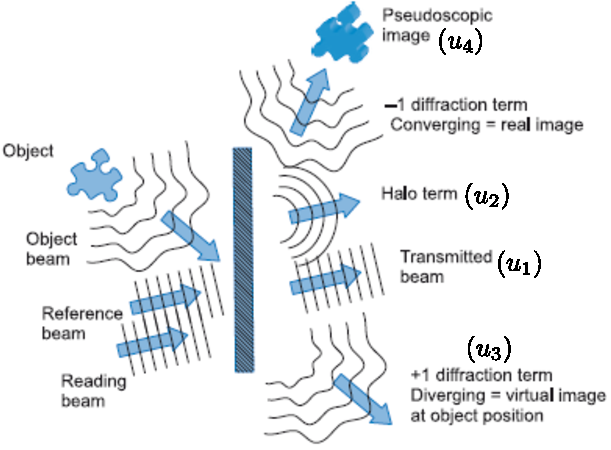
\includegraphics[width=0.4\textwidth]{./images/3-reconst}
	\label{fig:}
\end{figure}
%-----------------------------------------------------------------
% \newpage
\subsection{Difracció (teoria)}
\begin{align*}
	\laplacian2 U +kU^2=0 \tag{Helmholtz}
\end{align*}
Rayleigh--Sommerfeld: rere la l'apertura $U$ i $U'$ són iguals;  $U = U' \equiv 0$ rere la pantalla (zona opaca).
\begin{align*}
	U(P_{0}) =& \dfrac{z}{i\lambda}\iint_\Sigma  U(P_1)\dfrac{e^{ikr}}{r^2}\dd{\xi} \dd{\eta} \qc I(P_{0}) = U\sast(P_{0})U(P_{0})
\end{align*}
\subsubsection*{Aproximació de Fresnel (parabòlica)}
\begin{align*}\Scale[0.8]{%
	r = \sqrt{z^2+(x-\xi)^2+(y-\eta)^2} \approx z\left[1+\dfrac{1}{2}\left(\dfrac{x-\xi}{z}\right)^2+\dfrac{1}{2}\left(\dfrac{y-\eta}{z}\right)^2+ \cdots \right]
}\end{align*}
\begin{align*}\Scale[0.95]{%
	U(P_{0}) =\dfrac{ e^{ikz}}{iz\lambda} e^{\frac{ik}{2z}(x^2+y^2)}\iint_\Sigma  U(P_1) e^{-\frac{ik}{z}(y\eta+x\xi)} e^{\frac{ik}{2z}(\xi^2+\eta^2)}\dd{\xi} \dd{\eta}
}\end{align*}
\subsubsection*{Aproximació de Freaunhofer (ona plana)}
\begin{align*}
	F = \frac{a^{2}}{\lambda L}
	\begin{cases}
		\gtrsim 1 \Rightarrow \text{Fresnel} \\
		\ll 1 \Rightarrow \text{Fraunhofer} \,(z \gg \dfrac{k}{2}(\xi^{2} + \eta^{2}))
	\end{cases}
\end{align*}
\begin{align*} \Scale[0.98]{%
	% U(P_{0}) =\dfrac{ e^{ikz}}{iz\lambda} e^{\frac{ik}{2z}(x^2+y^2)}\iint_\Sigma  U(P_1) e^{-\frac{ik}{z}(y\eta+x\xi)} e^{\frac{ik}{2z}(\xi^2+\eta^2)}\dd{\xi} \dd{\eta}
	U(P_o) =\dfrac{ e^{ikz}}{iz\lambda} e^{\frac{ik}{2z}(x^2+y^2)}\iint_\Sigma  U(P_1) e^{-\frac{ik}{z}(y\eta+x\xi)} \dd{\xi} \dd{\eta} \Rightarrow \mc{F}
}\end{align*}

%-----------------------------------------------------------------
% \newpage
\subsection{Laboratori}
\begin{figure}[H]
	\centering
	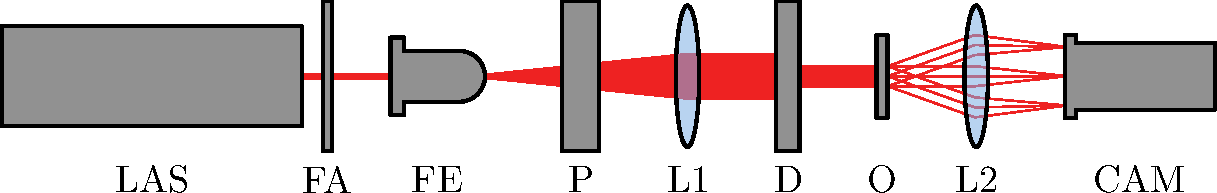
\includegraphics[width=0.5\textwidth]{./images/1-diagrama} \\ \vspace{1pt}
	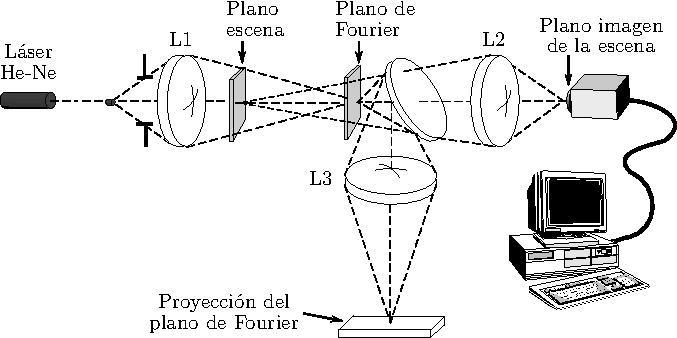
\includegraphics[width=0.5\textwidth]{./images/2-filtrado-esquema}
	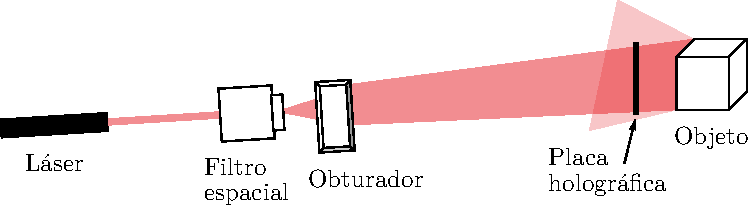
\includegraphics[width=0.5\textwidth]{./images/3-esquema}
	\label{fig:}
\end{figure}
